\section{Hallways, motions, and cap scores}\label{sec:setting}\label{sec:definitions}

We use $\abs{A}$ for two-dimensional Lebesgue measure and
$R_\theta$ for counterclockwise rotation by $\theta$. Put
\[
 u(\theta)=(\cos\theta,\sin\theta),\qquad
 u^\perp(\theta)=(-\sin\theta,\cos\theta),\qquad
 \refl(x,y)=(x,1-y).
\]
The reflection $\refl$ preserves the strip $\Strip=\R\times[0,1]$.

\begin{lemma}[Elementary bounds for the reference constant]\label{lem:constant-bounds}
The root and constant in \cref{eq:constant} satisfy
\[
 \frac{297}{1000}<Y<\frac3{10},\qquad
 \sqrt2<\frac85<\frac{41}{25}<\Mc.
\]
\end{lemma}
\begin{proof}
The polynomial $4y^3+3y$ is strictly increasing. Substitution at
$297/1000$ gives $248948073/250000000<1$, while its value at
$3/10$ is greater than one. For $y\ge0$,
$\arctan y\ge y-y^3/3$, since the derivative of
$\arctan y-y+y^3/3$ is $y^4/(1+y^2)\ge0$.
Using the cubic to replace $Y^3$ therefore gives
\[
 \Mc\ge\frac{11}{12}+4Y^2+\frac54Y
  >\frac{11}{12}+4(297/1000)^2+\frac54(297/1000)
  >\frac{41}{25}.
\]
The last inequality is rational arithmetic. The other comparisons
follow by squaring the positive quantities and comparing fractions.
\end{proof}

\subsection{The two passages}
The incoming and outgoing arms are
\begin{align*}
 \Hin&=(-\infty,1]\times[0,1],\\
 \Vm&=[0,1]\times(-\infty,1],&
 \Vp&=[0,1]\times[0,\infty).
\end{align*}
The two hallways are $\Lm=\Hin\cup\Vm$ and $\Lp=\Hin\cup\Vp$;
they are exchanged by $\refl$.

\begin{definition}\label{def:passage}
A passage of $S$ through $L=H\cup V$ consists of continuous maps
$\theta:[0,1]\to\R$ and $c:[0,1]\to\R^2$ such that
\[
 R_{\theta(0)}S+c(0)\subset H,\qquad
 R_{\theta(t)}S+c(t)\subset L\quad(0\le t\le1),\qquad
 R_{\theta(1)}S+c(1)\subset V.
\]
\end{definition}

\begin{definition}\label{def:ambidextrous}
An ambidextrous sofa is a nonempty compact connected set
$S\subset\R^2$ with a passage $(\theta_-,c_-)$ through $\Lm$ and
a passage $(\theta_+,c_+)$ through $\Lp$ satisfying
$R_{\theta_-(0)}=R_{\theta_+(0)}$.
\end{definition}

There is no smoothness assumption on $S$ or on either passage. The
continuous angle lifts may differ initially by an integer multiple of
$2\pi$. Compactness makes area finite, and connectedness refers to the
physical body, including its boundary. Initial translations need not
agree: translating a placement farther along the incoming arm does
not change its orientation.

\subsection{Caps and their roofs}
For a nonempty compact set $K$ define its support function by
\[
 h_K(\theta)=\max_{p\in K}\ip{p}{u(\theta)}.
\]
It is unchanged by taking the convex hull. For $K\subset\Strip$ let
\[
 K^\downarrow=\{(x,y):0\le y\le y'
              \text{ for some }(x,y')\in K\}.
\]

\begin{definition}\label{def:cap}
A downward cap is a nonempty compact convex set $U\subset\Strip$
such that $(x,y)\in U$ and $0\le y'\le y$ imply $(x,y')\in U$.
\end{definition}

Its horizontal projection is an interval $I_U=[l_U,r_U]$, its width
is $w_U=r_U-l_U$, and its roof is
\[
 f_U(x)=\max\{y:(x,y)\in U\}\quad(x\in I_U),
 \qquad f_U(x)=0\quad(x\notin I_U).
\]
On $I_U$ the roof is concave and takes values in $[0,1]$. The middle
half and exterior quarters are
\[
 J_U=[l_U+w_U/4,r_U-w_U/4],\qquad I_U\setminus J_U.
\]
The cap domain permits width zero, height less than one, flat faces,
and nonsmooth roofs. None of the later universal cap statements
assumes symmetry.

\subsection{The physical barrier}
Place a copy of $\Lm$ in the body's frame with its outer walls on
the supporting lines of $U$ with normals $u(\theta)$ and
$u^\perp(\theta)$. Its inner walls have heights
\begin{equation}\label{eq:walls}
 \begin{aligned}
 a_\theta(x)&=\frac{h_U(\theta)-1-x\cos\theta}{\sin\theta},\\
 b_\theta(x)&=\frac{h_U(\theta+\pi/2)-1+x\sin\theta}{\cos\theta}
 \qquad(0<\theta<\pi/2).
 \end{aligned}
\end{equation}
The forbidden open inner corner consists of points below both walls.
Its vertical threshold is $c_\theta(x)=\min(a_\theta(x),b_\theta(x))$.

For $0<\alpha\le\pi/2$ define the swept niche and full partial barrier
by
\begin{align}
 n_\alpha(U)(x)&=\max\left(0,\sup_{0<\theta<\alpha}c_\theta(x)\right),
       \label{eq:niche}\\
 N_\alpha(U)(x)&=\max\bigl(n_\alpha(U)(x),a_\alpha(x)\bigr).
       \label{eq:barrier}
\end{align}
The first-wall formula in \cref{eq:walls} remains defined at
$\alpha=\pi/2$. There
$a_{\pi/2}(x)=h_U(\pi/2)-1\le0$, so
$N_{\pi/2}(U)=n_{\pi/2}(U)$. At a proper terminal angle the outgoing
strip requires $y\ge a_\alpha(x)$ over the entire body, including
abscissae where that wall lies above the two-ray niche. This is why
the terminal wall appears separately in \cref{eq:barrier}.

\begin{lemma}[Continuity of the barrier]\label{lem:barrier-continuity}
For every downward cap $U$, $n_\alpha(U)$ and $N_\alpha(U)$
are continuous functions of $x$ for $\pi/4\le\alpha\le\pi/2$.
They are bounded and integrable on the cap's projection interval.
\end{lemma}
\begin{proof}
Set
\[
 \begin{aligned}
 m_U(x,t)&=\bigl(\min\{a_t(x),b_t(x)\}\bigr)_+
       &&(0<t<\pi/2),\\
 m_U(x,0)&=m_U(x,\pi/2)=0.
 \end{aligned}
\]
where $z_+=\max(z,0)$. On the open angular interval this is
continuous. At $t=0$, use
\[
 0\le m_U(x,t)\le
 \left(\frac{h_U(t+\pi/2)-1+x\sin t}{\cos t}\right)_+.
\]
The right side tends to zero, locally uniformly in $x$, because
$h_U(\pi/2)\le1$. At $t=\pi/2$ the analogous bound by
$(a_t(x))_+$ tends to zero. Thus $m_U$ is continuous on
$\R\times[0,\pi/2]$. Continuity at a proper terminal angle also
shows that
\[
 n_\alpha(U)(x)=\max_{0\le t\le\alpha}m_U(x,t).
\]
A continuous function's maximum over a compact interval depends
continuously on $x$: uniform continuity on any compact rectangle
bounds the difference of the two maxima by the largest difference
of the corresponding values. The terminal wall $a_\alpha$ is
continuous, since $\sin\alpha>0$, so taking its maximum with
$n_\alpha(U)$ proves the claim for $N_\alpha(U)$.
\end{proof}

\begin{figure}[htbp]
 \centering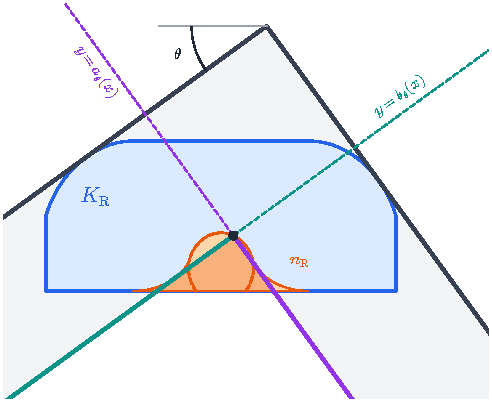
\includegraphics[width=.86\textwidth]{figures/fig-walls.pdf}
 \caption{The supporting hallway at $\theta=\pi/5$ for Romik's cap.
 The inner walls meet at its moving corner. The dashed corner path
 sweeps the niche as the angle varies.}\label{fig:walls}
\end{figure}

\begin{definition}\label{def:score}
The score of a cap at angle $\alpha$ is
\begin{equation}\label{eq:cap-score}
 P_\alpha(U)=\int_{I_U\setminus J_U}f_U(x)\,\dd x
              -\int_{J_U}N_\alpha(U)(x)\,\dd x.
\end{equation}
\end{definition}

The middle roof contributes no positive term to the score; its
support lines still affect the barrier. Both integration domains
move when the cap's projection changes. The elementary bound
\begin{equation}\label{eq:half-width}
 P_\alpha(U)\le w_U/2
\end{equation}
follows from $f_U\le1$, $N_\alpha(U)\ge0$, and
$\abs{I_U\setminus J_U}=w_U/2$.

\begin{figure}[htbp]
 \centering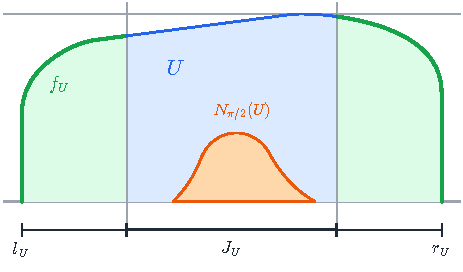
\includegraphics[width=.84\textwidth]{figures/fig-score.pdf}
 \caption{The score counts the roof over the two outer quarters
 (green) and subtracts the barrier over the middle half (orange).
 The cap drawn here is a generic cap, rather than Romik's.}\label{fig:score}
\end{figure}
